\chapter{Conference Customization Prototype} \label{chap:conference_customization_prototype}

    Gli eventi, ed in particolare le conferenze, sono un concetto centrale in Indico e, come tale, rivestono un ruolo molto importante nell'utilizzo dell'applicazione. È quindi altrettanto importante fornire agli utenti uno strumento che sia in grado di assisterli durante la creazione e la personalizzazione di una conferenza, così che, in modo semplice e intuitivo, l'utente possa creare delle pagine di conferenze belle, moderne e funzionali.
    
    \begin{figure}[h!]
        \begin{center}
    		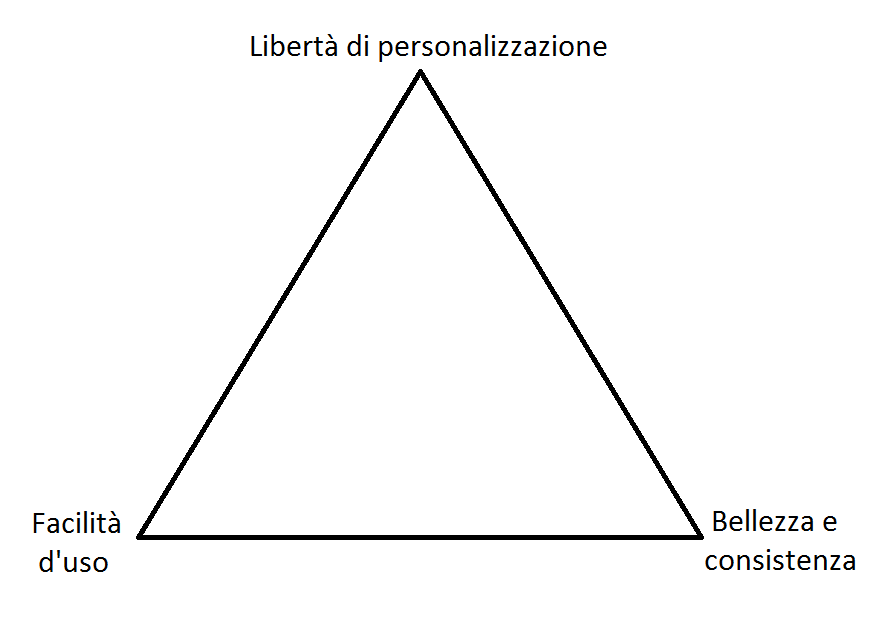
\includegraphics[scale=0.8]{conference_triangle.png}
    	\end{center}
        \caption[Caratteristiche di un tool di personalizzazione di conferenze]{Caratteristiche desiderate in un tool di personalizzazione di conferenze.}
        \label{fig:conference_triangle}
    \end{figure}
    
    In Figura \ref{fig:conference_triangle} vediamo schematizzate le principali caratteristiche che vorremmo uno strumento di personalizzazione di conferenze avesse, che descriviamo qui di seguito:
    
    \begin{itemize}
        \item \textbf{Libertà di personalizzazione}: il tool deve garantire quanta più libertà di personalizzazione, per permettere all'utente di realizzare il più possibile la sua idea di conferenza, adattandola alle sue esigenze e gusti personali;
        \item \textbf{Facilità d'uso}: il tool dev'essere il più facile e intuitivo possibile da utilizzare: è inutile, infatti, mettere l'utente di fronte a una sfilza di bottoni e strumenti se poi l'utente ne utilizzerà soltanto due o tre perché non conosce il significato degli altri;
        \item \textbf{Bellezza e consistenza}: il tool deve favorire la creazione di pagine di conferenze che abbiano uno stile moderno e consistente e, allo stesso tempo, rendere difficile (se non impossibile) la creazione di pagine antiestetiche.
    \end{itemize}
    
    Chiaramente, la situazione ideale sarebbe avere tutte e tre le caratteristiche presenti nel tool di personalizzazione, tuttavia, come vedremo più avanti, non sarà possibile trovare un tool simile e sarà necessario scendere a compromessi.
    
    Prima di iniziare a parlare del tool sviluppato in questa fase del progetto, vediamo prima brevemente qual è la situazione attuale per quanto riguarda la personalizzazione di conferenze in Indico.
    
    \section{Situazione attuale} \label{sec:ccp;situazione_attuale}
    
        La situazione del tool per la personalizzazione di conferenze prima dell'inizio del progetto (e tutt'ora al momento della stesura di questa tesi) era che questo strumento permetteva di creare eventi piuttosto gradevoli e consistenti con lo stile di Indico. Un esempio può essere la conferenza in Figura \ref{fig:conference_old}, della quale possiamo notare lo stile minimale e l'utilizzo di icone consistenti con lo stile di Indico e del \ac{CERN} in generale.
        
        \begin{figure}[h!]
            \begin{center}
        		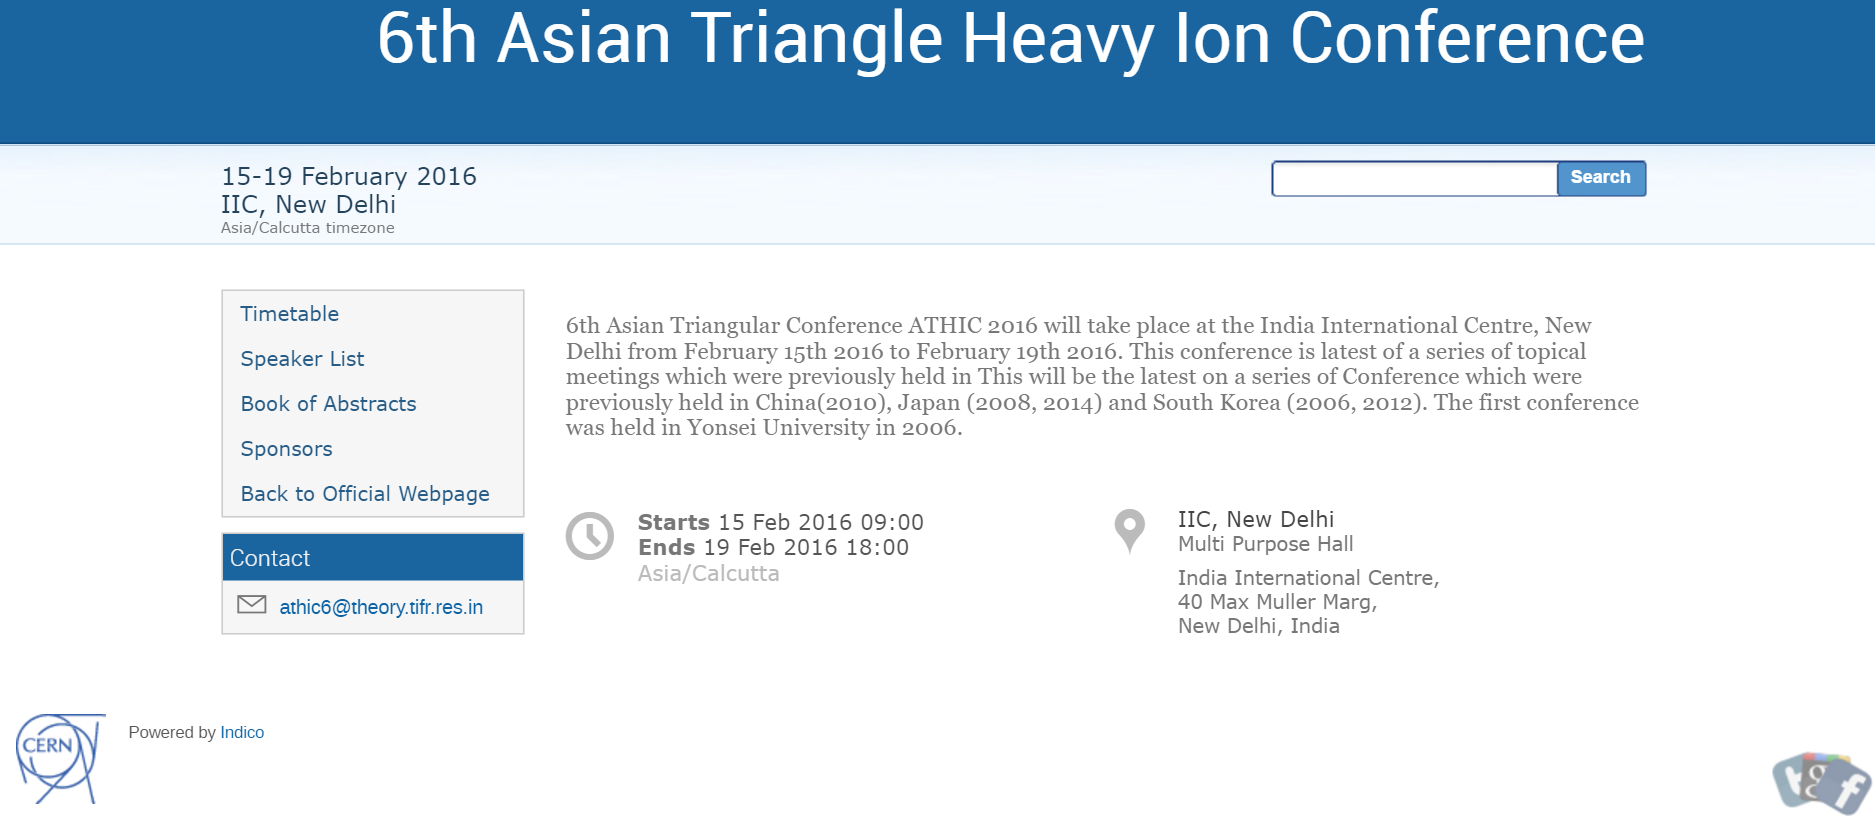
\includegraphics[scale=0.4]{conference_old.png}
        	\end{center}
            \caption[Esempio di conferenza in Indico]{Esempio della situazione attuale delle conferenze in Indico (fonte \url{https://indico.cern.ch/event/487533/}).}
            \label{fig:conference_old}
        \end{figure}
        
        Lo stile, tuttavia, risulta essere non troppo moderno: molte pagine di conferenze su Internet utilizzano elementi dinamici e interattivi ed uno stile, in generale, più moderno.
        
        Per quanto riguarda il tool di personalizzazione vero e proprio, c'è da dire che esso non permette una piena libertà di personalizzazione, mettendo a disposizione dell'utente soltanto pochi stili ed elementi di layout. Inoltre molte opzioni e possono risultare, per l'utente medio, difficili da utilizzare o poco intuitive, anche per il fatto che l'interfaccia non è molto user-friendly, come possiamo vedere in Figura \ref{fig:conference_customization}.
        
        \begin{figure}[h!]
            \begin{center}
        		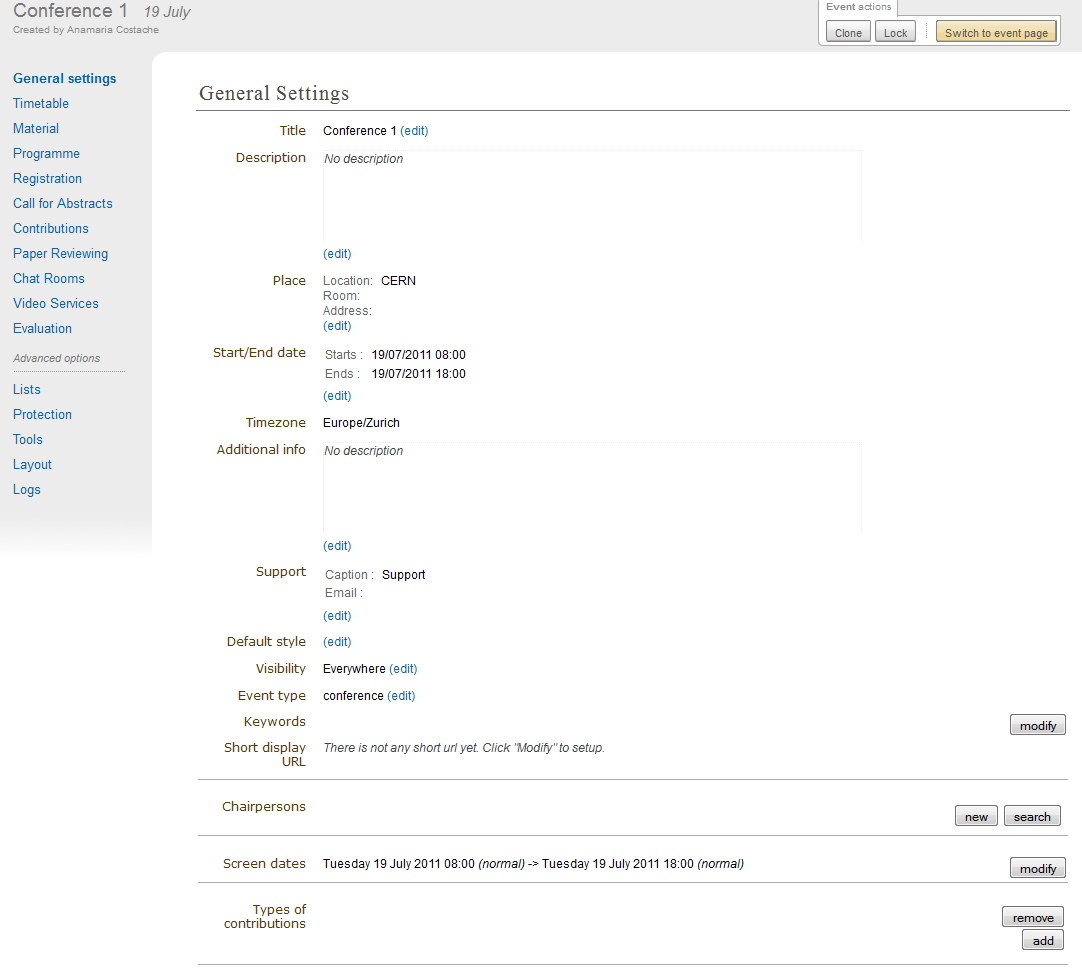
\includegraphics[scale=0.7]{conference_customization.png}
        	\end{center}
            \caption[Tool di configurazione di una conferenza in Indico]{Interfaccia della pagina di configurazione di una conferenza in Indico.}
            \label{fig:conference_customization}
        \end{figure}
        
        Quindi Indico permette di creare pagine di conferenze con stili gradevoli e consistenti, al costo di limitare ampiamente la libertà di personalizzazione, il tutto utilizzando un'interfaccia di personalizzazione non sempre intuitiva.
        
        Tra le opzioni avanzate del tool di personalizzazione, era inoltre presente la possibilità di far caricare all'utente il proprio stile \ac{CSS}. Sfruttando quest'opzione l'utente è in grado di avere pieno controllo sulla personalizzazione della pagina, potendo definire il proprio stile \ac{CSS} in maniera totalmente libera. Tuttavia quest'approccio ha due problemi principali: è complicato da utilizzare, per l'utente medio, e permette all'utente di creare qualsiasi tipo di pagina, comprese pagine brutte, inconsistenti o, in generale, antiestetiche.
        
        \subsection{La necessità di un nuovo strumento} \label{subsec:ccp;sa;necessità_nuovo_strumento}
        
            In questo progetto finale del Progetto KT si è allora cercato di sviluppare un prototipo per un tool di creazione e personalizzazione di conferenze.
            
            Si parla di prototipo in quanto a questa fase sono stati dedicati, da contratto, soltanto gli ultimi mesi del programma di Technical Student oggetto di questa tesi, che sono stati considerati del tutto insufficienti, a priori, per sviluppare un prodotto finito. Inoltre, prima di iniziare lo sviluppo vero e proprio di un tool di personalizzazione di conferenze, era necessario capire in che direzione si voleva portare questo futuro tool, ovvero che forma e caratteristiche dovesse avere. Quest'ultima fase del Progetto KT è stata quindi incentrata proprio su questo: indagare e investigare tutte le possibili soluzioni per un futuro tool di personalizzazione di conferenze sviluppando, a supporto del processo di analisi, un prototipo che rispecchiasse, di volta in volta, le idee proposte\footnote{Il codice aggiornato del progetto può essere consultato all'interno del repository GitHub \url{https://github.com/indico/conference-customization-2.0}}.
            
            Questo progetto è stato quindi più un progetto di indagine, riguardo a come strutturare un tool futuro, che di sviluppo. Per questo ci concentreremo, nel seguito della trattazione, su aspetti decisionali e sui vari step che hanno composto questa fase, piuttosto che su aspetti tecnici. Infatti il codice del prototipo sviluppato non verrà utilizzato in alcun modo per lo sviluppo del tool finale, che verrà scritto da zero, probabilmente con i fondi di un secondo Progetto KT per Indico. In ogni caso, il codice del prototipo sviluppato al \ac{CERN} negli ultimi mesi è disponibile al seguente repository GitHub: \url{https://github.com/indico/conference-customization-2.0}.
            
            In generale, i possibili approcci che si potevano intraprendere per la personalizzazione di conferenze erano tre:
            
            \begin{itemize}
                \item \textbf{Approccio alla Facebook}: creare uno stile molto bello, molto carino e consistente ma fornire un solo stile unico uguale per tutti; quest'approccio risulterebbe molto semplice da gestire, ma non fornirebbe alcun tipo di personalizzazione all'utente;
                \item \textbf{Upload di \ac{CSS}}: come l'opzione avanzata già presente in Indico al momento, permettere di caricare i propri stili \ac{CSS} personali permette all'utente di personalizzare la pagina come più gli piace, ma gli dà anche la libertà di creare conferenze antiestetiche o inconsistenti (il problema della consistenza è importante in quanto l'organizzazione che gestisce l'istanza di Indico ha una certa immagine da rispettare ed una pagina brutta o con stile diverso si può riflettere negativamente sull'immagine dell'organizzazione);
                \item \textbf{Approccio orientato ai widget}: definire un insieme finito di tipi di widget (come negli smartphone) che l'utente può posizionare nella pagina e personalizzare, entro un certo limite.
            \end{itemize}
            
            Chiaramente le prime due soluzioni rappresentano i due casi estremi in cui si punta tutto alla bellezza e alla consistenza, da un lato, e in cui si punta tutto sulla libertà di personalizzazione, dall'altro. Il terzo approccio è invece un approccio ibrido ed è stata l'opzione che, fin dal principio, è sembrata essere la più promettente e sensata delle tre.
            
            Questa progetto è quindi stato composto da una serie di prove ed errori, idee e suggerimenti, ognuno dei quali veniva proposto all'intero team di Indico durante ogni meeting, che si teneva regolarmente ogni settimana, per decidere se valeva la pena continuare ad investigare in quella direzione o se era necessario un cambio di programma. Spesso infatti il prototipo è stato riscritto quasi da zero. Molte altre volte le modifiche sono invece state minime e graduali, cambiando il prototipo a poco a poco.
            
            Per queste ragioni, nelle Sezioni successive, non mostreremo tutti i singoli passi attraverso i quali il prototipo si è evoluto, ma soltanto i due principali checkpoint dello sviluppo, che rappresentano i due approcci che sono stati principalmente indagati durante questa fase.
            
    \section{Classi di widget} \label{sec:ccp;classi_widget}
    
        Fin da subito l'idea di indagare una soluzione orientata ai widget è piaciuta all'intero team di Indico. Con widget si intendono parti del layout indipendenti, riusabili e componibili. Il primo obiettivo è stato quindi definire, a grandi linee, le classi di widget che si volevano includere nel tool di personalizzazione e, per ognuna di esse, dare un'idea generale di come si poteva personalizzare e come avrebbe dovuto comportarsi.
        
        Alcuni widget avrebbero ripreso la funzione di alcune parti della vecchia pagina delle conferenze presente in Indico, come ad esempio si è pensato subito ad un widget per mostrare la timetable della conferenza, o ancora un widget che visualizzasse il luogo dell'evento. Altri widget invece sono stati ideati sul momento, tramite i suggerimenti di tutti i membri del team e attraverso svariate sessioni di brainstorming.
        
        Di seguito proponiamo la lista delle classi di widget ideate durante questa fase, con tanto di descrizione. Le classi di widget proposte sono state suddivise in due classi: widget generici, che possono essere usati per molti fini diversi tra loro ed il cui utilizzo dipende dall'utente, e widget dedicati, che invece sono più specializzati ed hanno uno scopo ben preciso. Nelle Figure dalla \ref{fig:list} alla \ref{fig:menu_vertical} possiamo vedere alcuni degli sketch abbozzati durante le prime fasi di brainstorming con l'intero team per avere meglio un'idea di come sarebbero apparsi, graficamente, i vari widget, in modo da decidere quali classi di widget includere e quindi strutturare la pagina in modo adeguato.
        
        \begin{itemize}
            \item Widget generici
                \begin{itemize}
                    \item \textbf{Lista}: una generica lista di elementi testuali, come una frase, una descrizione o informazioni utili (Figura \ref{fig:list} lo stile prevedeva la scelta del bordo (con o senza), la possibilità di aggiungere un titolo e la possibilità di formattare il testo, ad esempio inserendo elenchi puntati o icone;
                    \item \textbf{Carosello}: una serie di elementi grafici o testuali che si alternano, scorrendo orizzontalmente; la scelta dello stile includeva la selezione di un'immagine di sfondo, la possibilità di visualizzare un elemento alla volta (Figura \ref{fig:carousel_single-element}) o più di uno (Figura \ref{fig:carousel_multi-element}), l'aggiunta di un titolo, la possibilità di mostrare o meno una breve descrizione sotto ogni elemento e la possibilità di avere delle frecce o bottoni di navigazione; questo tipo di widget può essere utilizzato per mostrare gli argomenti principali di una conferenza, o i principali sponsor, o semplicemente come galleria fotografica;
                    \item \textbf{Riquadro}: un widget generico (Figura \ref{fig:box}) che può contenere elementi testuali, grafici o una combinazione dei due, ad esempio utilizzandolo come titolo per una conferenza o per mostrare avvisi importanti; lo stile prevede la scelta del bordo e del titolo, nonché del contenuto.
                \end{itemize}
            \item Widget dedicati
                \begin{itemize}
                    \item \textbf{Date}: widget che mostra le date principali dell'evento; lo stile può essere sotto forma di lista o di carosello; l'idea era di poter caricare le date di inizio e fine dell'evento direttamente dal database di Indico e allo stesso tempo dare la possibilità all'utente di aggiungere dare aggiuntive;
                    \item \textbf{Luogo}: widget che mostra il luogo fisico in cui si tiene la conferenza; lo stile prevede una mappa (tramite le \ac{API} di Google Maps o tramite immagine, come in Figura \ref{fig:map}), un indirizzo, delle indicazioni stradali oppure una combinazione delle tre cose (Figura \ref{fig:map_address_directions}); come prima, l'idea era di caricare il luogo direttamente da Indico ed eventualmente aggiungere mappe extra;
                    \item \textbf{Materiale}: widget per visualizzare tutto il materiale caricato nella pagina dell'evento; lo stile può essere sia lista che carosello; l'idea era di caricare i file presenti dal database ed eventualmente associare ad ognuno di essi un'azione (apri/scarica/ecc\dots);
                    \item \textbf{Persone coinvolte}: un elenco di persone coinvolte nella conferenza (ad esempio autori o speaker) sotto forma di lista o carosello;
                    \item \textbf{Condivisione su social media}: una serie di bottoni per condividere in modo rapido la pagina dell'evento tramite i principali social media, come Facebook, Twitter o Google+; il widget è stato pensato in versione sia orizzontale (Figura \ref{fig:share_horizontal}) che verticale (Figura \ref{fig:share_vertical}) e con la possibilità di aggiungere accanto ad ogni bottone il numero di condivisioni tramite quel particolare social media;
                    \item \textbf{Notizie tramite social media}: ultime notizie caricate dalla pagina relativa alla conferenza su un particolare social media (Figura \ref{fig:social_media_news}); in questo caso l'utente dovrebbe specificare da quale account/pagina caricare le notizie da visualizzare;
                    \item \textbf{Menu}: semplice menu, orizzontale (Figura \ref{fig:menu_horizontal}) o verticale (Figura \ref{fig:menu_vertical}), con bottoni e la possibilità di aggiungere sotto-menu innestati;
                    \item \textbf{Titolo}: un widget orizzontale, largo quanto tutta la pagina, contenente il titolo della conferenza e uno sfondo scelto dall'utente;
                    \item \textbf{Ricerca}: barra di ricerca di Indico o di Google;
                    \item \textbf{Timetable}: widget dedicato alla timetable della conferenza.
                \end{itemize}
        \end{itemize}
        
       	\begin{figure}[h!]
       		\begin{center}
       			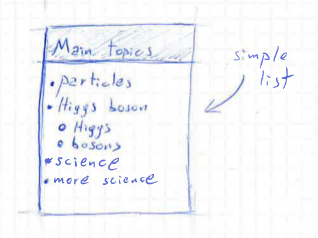
\includegraphics[scale=0.6]{list.png}
       		\end{center}
       		\caption[Sketch del widget ``lista'']{Sketch del widget ``lista''.}
       		\label{fig:list}
       	\end{figure}
       	
       	\begin{figure}[h!]
       		\begin{center}
       			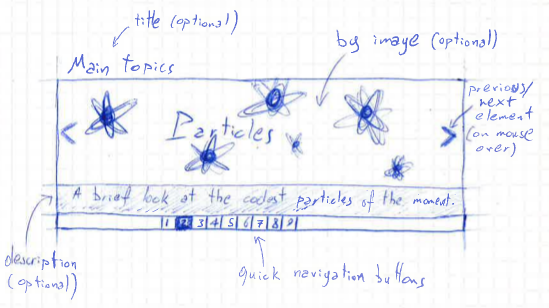
\includegraphics[scale=0.5]{carousel_single-element.png}
       		\end{center}
       		\caption[Sketch del widget ``carosello'' (elemento singolo)]{Sketch del widget ``carosello'' con un solo elemento a volta.}
       		\label{fig:carousel_single-element}
       	\end{figure}
        
       	\begin{figure}[h!]
       		\begin{center}
       			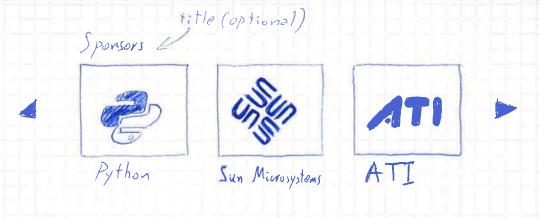
\includegraphics[scale=0.6]{carousel_multi-element.png}
       		\end{center}
       		\caption[Sketch del widget ``carosello'' (elementi multipli)]{Sketch del widget ``carosello'' con più elementi a volta.}
       		\label{fig:carousel_multi-element}
       	\end{figure}
        
       	\begin{figure}[h!]
       		\begin{center}
       			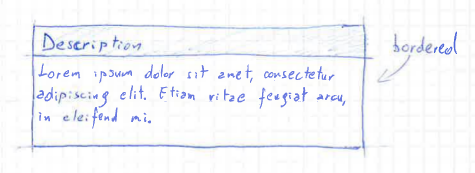
\includegraphics[scale=0.6]{box.png}
       		\end{center}
       		\caption[Sketch del widget ``riquadro'']{Sketch del widget ``riquadro''.}
       		\label{fig:box}
       	\end{figure}
       	
       	\begin{figure}[h!]
       		\begin{center}
       			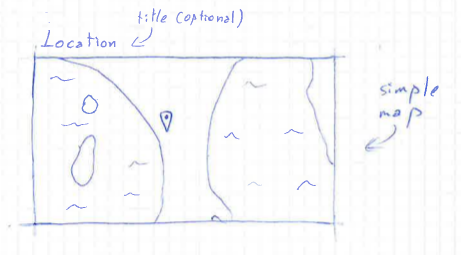
\includegraphics[scale=0.6]{map.png}
       		\end{center}
       		\caption[Sketch del widget ``luogo'' (semplice)]{Sketch del widget ``luogo'' con la sola mappa.}
       		\label{fig:map}
       	\end{figure}
       	
       	\begin{figure}[h!]
       		\begin{center}
       			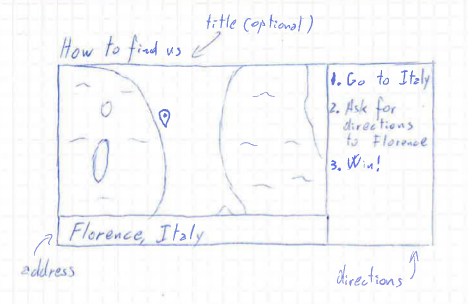
\includegraphics[scale=0.6]{map_address_directions.png}
       		\end{center}
       		\caption[Sketch del widget ``luogo'' (con indirizzo e indicazioni)]{Sketch del widget ``luogo'' con mappa, indirizzo e indicazioni stradali.}
       		\label{fig:map_address_directions}
       	\end{figure}
       	
       	\begin{figure}[h!]
       		\begin{center}
       			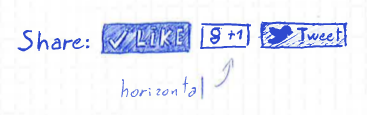
\includegraphics[scale=0.6]{share_horizontal.png}
       		\end{center}
       		\caption[Sketch del widget ``condivisione su social media'' (orizzontale)]{Sketch del widget ``condivisione su social media'' in formato orizzontale.}
       		\label{fig:share_horizontal}
       	\end{figure}
       	
       	\begin{figure}[h!]
       		\begin{center}
       			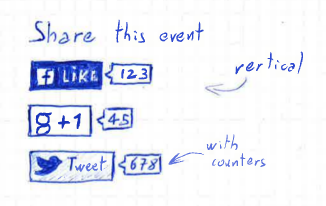
\includegraphics[scale=0.6]{share_vertical.png}
       		\end{center}
       		\caption[Sketch del widget ``condivisione su social media'' (verticale)]{Sketch del widget ``condivisione su social media'' in formato verticale.}
       		\label{fig:share_vertical}
       	\end{figure}
       	
       	\begin{figure}[h!]
       		\begin{center}
       			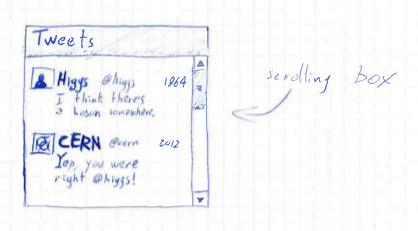
\includegraphics[scale=0.6]{social_media_news.png}
       		\end{center}
       		\caption[Sketch del widget ``notizie tramite social media'']{Sketch del widget ``notizie tramite social media''.}
       		\label{fig:social_media_news}
       	\end{figure}
       	
       	\begin{figure}[h!]
       		\begin{center}
       			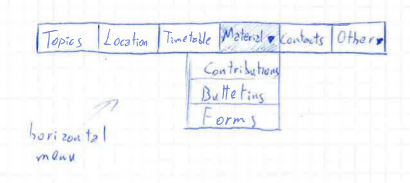
\includegraphics[scale=0.6]{menu_horizontal.png}
       		\end{center}
       		\caption[Sketch del widget ``menu'' (orizzontale)]{Sketch del widget ``menu'' in formato orizzontale.}
       		\label{fig:menu_horizontal}
       	\end{figure}
       	
       	\begin{figure}[h!]
       		\begin{center}
       			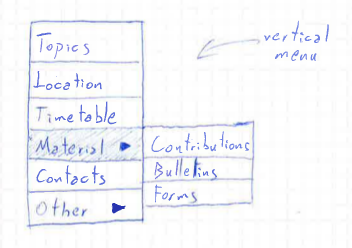
\includegraphics[scale=0.6]{menu_vertical.png}
       		\end{center}
       		\caption[Sketch del widget ``menu'' (verticale)]{Sketch del widget ``menu'' in formato verticale.}
       		\label{fig:menu_vertical}
       	\end{figure}
       	
       	\FloatBarrier
       	
    \section{User Interface} \label{sec:ccp;user_interface}
    
        Durante le prime fasi di brainstorming al \ac{CERN} si sono anche definiti alcuni elementi base dell'interfaccia utente che si volevano includere nella versione finale del progetto.
        
        L'idea era quella di progettare uno strumento di personalizzazione di conferenze che fosse facile e intuitivo da usare. Rimanendo sulla scia di idee dei widget, uno dei concetti chiave che sono emersi è stata la possibilità di avere un'interfaccia basata sul drag-and-drop, ovvero poter piazzare gli widget all'interno della pagina semplicemente trascinandoli col mouse e, in generale, poterli personalizzare tramite pochi click. Si era infatti pensato anche che, in fase di personalizzazione della pagina, sopra ogni widget sarebbe potuta comparire una serie di bottoni per la modifica e personalizzazione dello widget, in modo da mantenere ogni widget graficamente separato dall'altro (anche in fase di modifica) e di rendere l'intero processo il più intuitivo possibile.
       	
    \section{Approccio a widget totale} \label{sec:ccp;approccio_widget_totale}
    
        Una volta definite le classi di widget da includere, ovvero i ``mattoni'' elementari che avrebbero composto la pagina delle conferenze, si è iniziato a pensare a come strutturare la pagina di una conferenza, ovvero come gestire questi widget.
        
        Il primo approccio perseguito prevedeva una struttura della pagina successivamente denominata \textit{full widget-based layout}, ovvero ``struttura totalmente orientata ai widget''. Questo approccio prevedeva di rappresentare la pagina delle conferenze tramite un'enorme griglia che dividesse la pagina in tanti spazi vuoti: in ognuno di questi spazi l'utente avrebbe potuto piazzare un widget ed eventualmente ridimensionarlo a piacimento in modo da fargli occupare più spazi. La suddivisione orizzontale starebbe stata fissa, mentre gli spazi sarebbero potuti estendersi all'infinito in senso verticale. Inoltre erano stati ideati dei contenitori, con lo scopo di poter raggruppare al loro interno widget o altri contenitori.
        
        In Figura \ref{fig:full_widget_layout} vediamo lo sketch abbozzato durante lo studio di questo approccio, per poter essere presentato al resto del team in fase di meeting.
        
       	\begin{figure}[h!]
       		\begin{center}
       			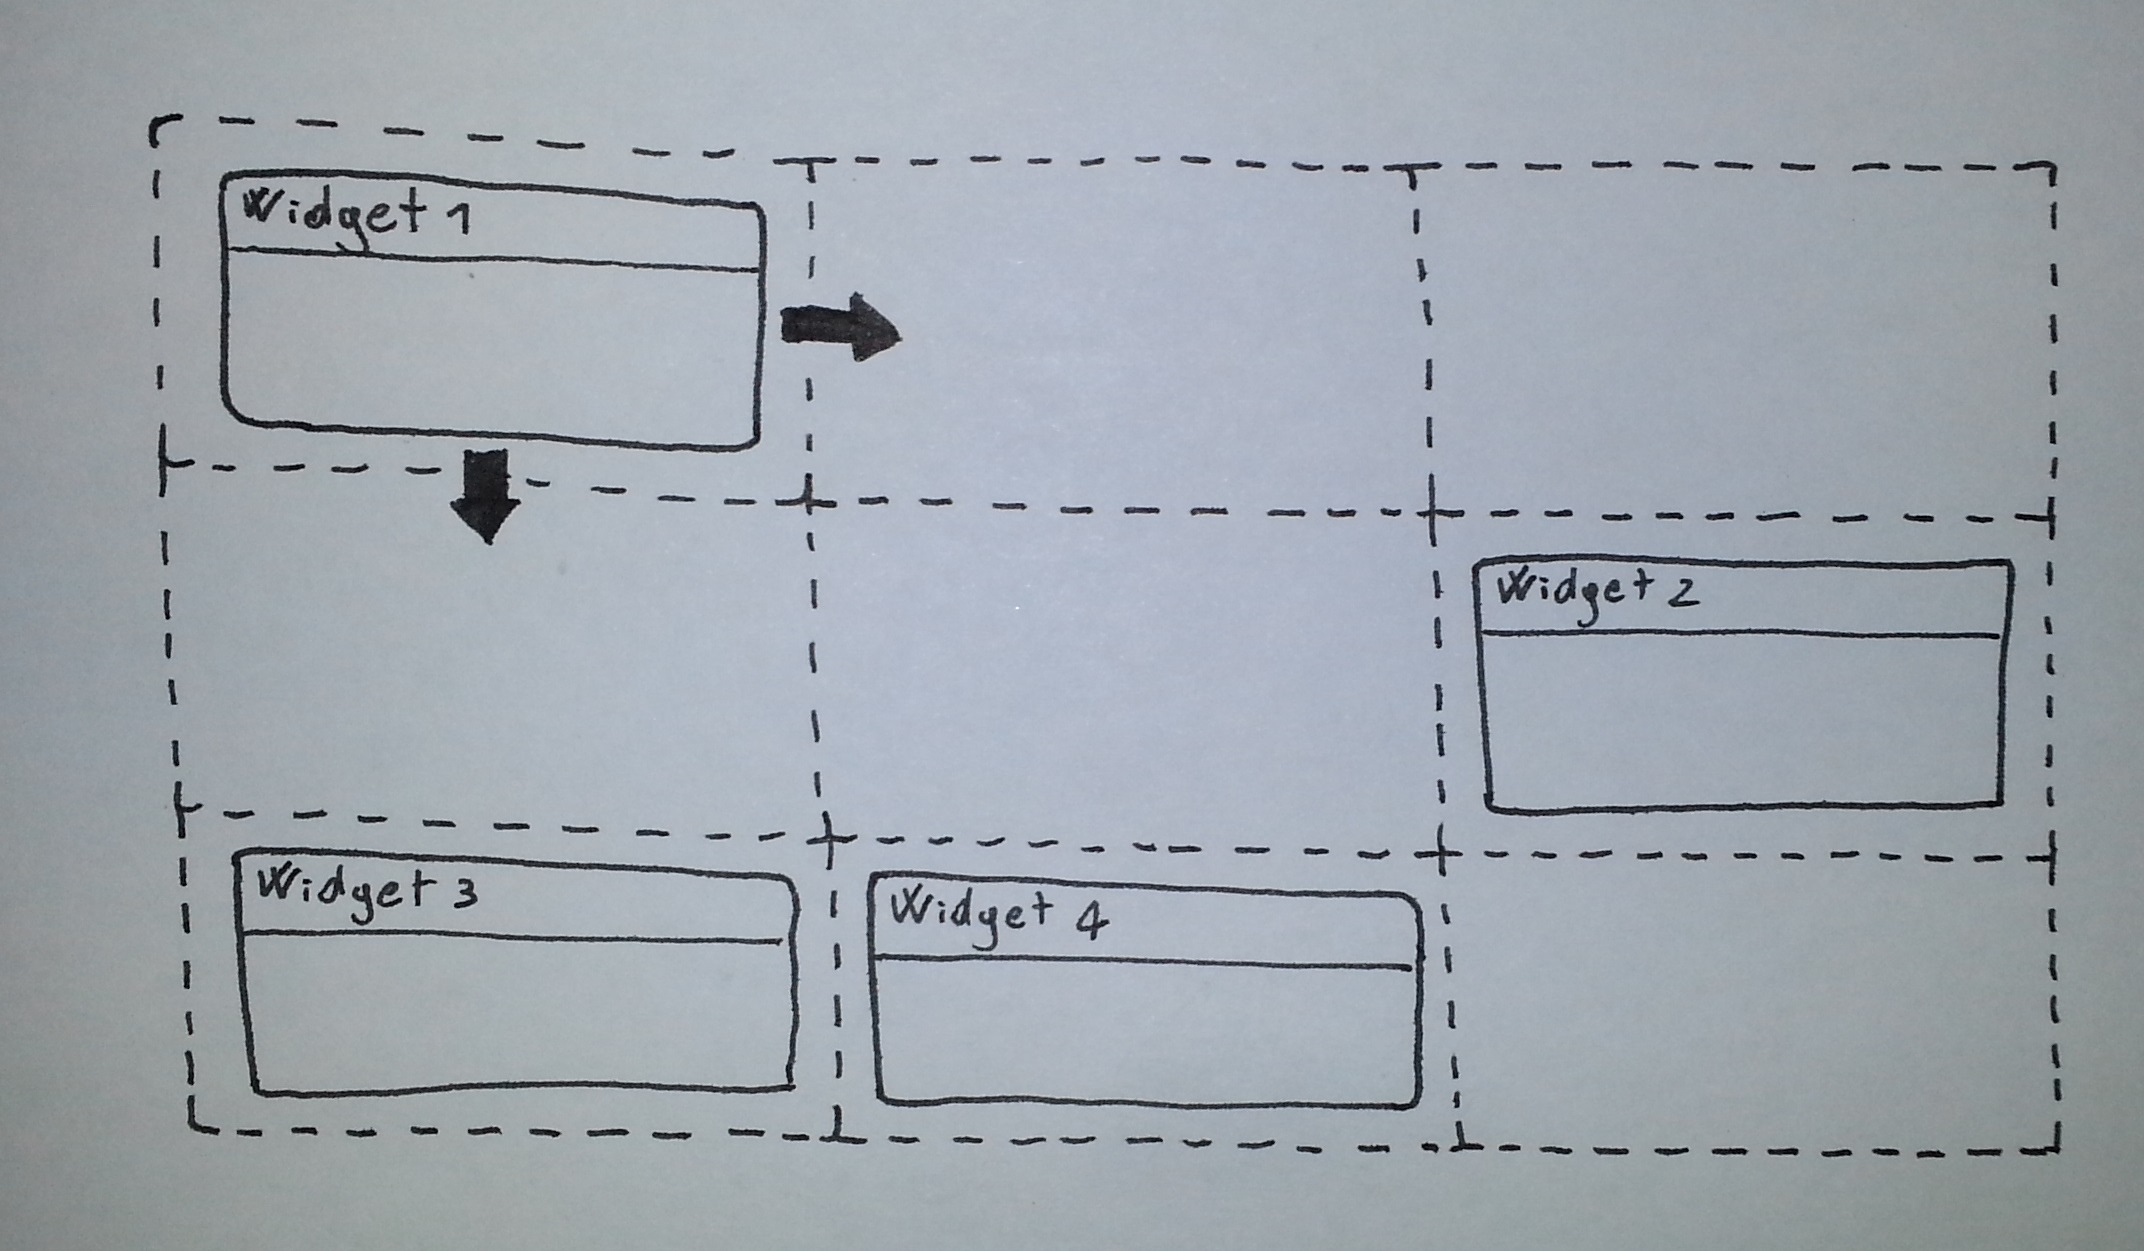
\includegraphics[scale=0.15]{full_widget_layout.jpg}
       		\end{center}
       		\caption[Sketch della struttura a widget totale]{Sketch del funzionamento della struttura totalmente orientata ai widget.}
       		\label{fig:full_widget_layout}
       	\end{figure}
       	
       	L'idea di poter creare uno strumento orientato ai widget e dotato di interfaccia drag-and-drop ha tuttavia fatto perdere di vista il fatto che, con una struttura del genere, veniva data all'utente troppa libertà di personalizzazione, forse in grado anche peggiore rispetto all'upload dello stile \ac{CSS} (come avviene attualmente in Indico). Infatti con questa struttura era possibile creare pagine molto brutte e instabili, ad esempio creando widget giganteschi che occupassero tutta la pagina, o creando serie di contenitori innestati, rendendo illeggibile il contenuto. Inoltre anche solo il fatto di poter piazzare gli widget ovunque l'utente desiderasse incoraggiava la creazione di pagine inconsistenti e senza un ordine logico preciso.
       	
       	Il problema di questo approccio era quindi che, nonostante si utilizzassero un'interfaccia drag-and-drop e elementi basati su widget per rendere lo stile più moderno, l'utente aveva ancora troppa libertà di personalizzazione, rischiando di creare pagine altamente antiestetiche e inutilizzabili.
    
    \section{Approccio a widget ibrido} \label{sec:ccp;approccio_widget_ibrido}
    
        Dopo molte sessioni di brainstorming, durante le quali sono state fatte molte proposte per risolvere il problema della struttura totalmente orientata ai widget, e dopo molte modifiche al prototipo, si è raggiunto un consenso con la struttura detta \textit{block-widget hybrid layout}, ovvero ``struttura ibrida basata su blocchi e widget''.
        
        L'idea di base di questo approccio è di suddividere la pagina verticalmente in sezioni, che occupano l'intera larghezza della pagina. Ognuna di queste sezioni è detta \textit{blocco} e rappresenta una sezione della pagina dove viene definito un unico stile di formattazione. All'interno del blocco possono essere messi dei widget, ordinandoli orizzontalmente o verticalmente, a seconda del blocco scelto.
        
       	\begin{figure}[h!]
       		\begin{center}
       			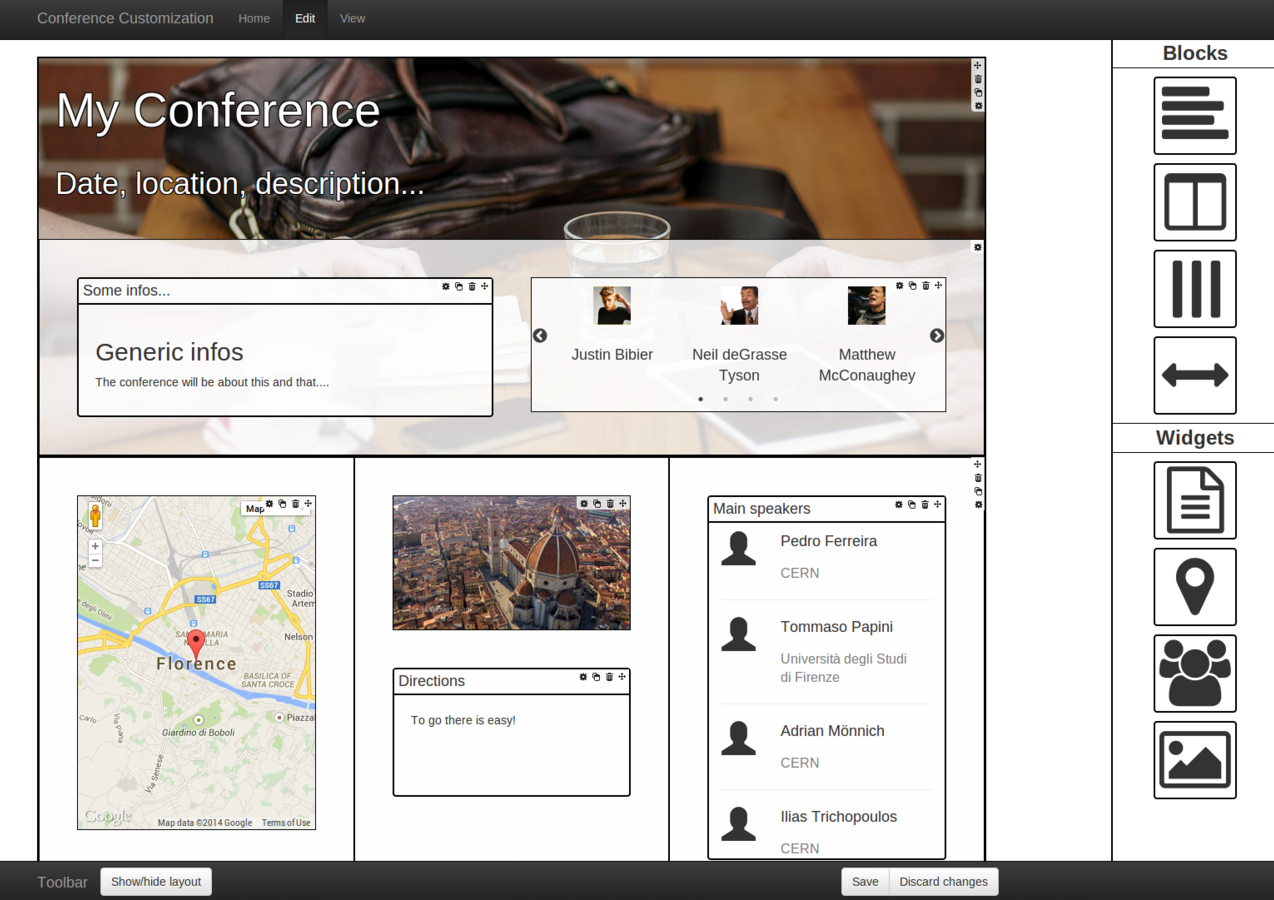
\includegraphics[scale=0.5]{prototype.png}
       		\end{center}
       		\caption[Versione finale del prototipo]{Schermata d'esempio della versione finale del prototipo.}
       		\label{fig:prototype}
       	\end{figure}
       	
       	In Figura \ref{fig:prototype} vediamo una schermata rappresentativa del prototipo costruito seguendo la struttura di quest'ultimo approccio, ovvero una struttura ibrida con widget e blocchi. Sulla destra possiamo vedere una barra contenente i blocchi e i widget implementati. I blocchi disponibili sono: colonna singola, due colonne, tre colonne o blocco orizzontale. Gli widget invece sono: riquadro testuale, luogo (con mappa tramite Google Maps), persone coinvolte o immagine. Per ogni widget e per ogni blocco possiamo notare, nell'angolo in alto a destra, quattro icone che servono, intuitivamente, per personalizzare, duplicare, eliminare o trascinare quel widget o blocco. Tutta l'interfaccia del prototipo in quest'ultima fase supportava pienamente il drag-and-drop e, cliccando sul pulsante per la personalizzazione di un widget/blocco, si apriva un riquadro popup sullo schermo con i campi relativi a quell'elemento che l'utente può modificare.
       	
       	Tirando le conclusioni, quest'ultimo approccio combina la facilità di utilizzo (tramite interfaccia drag-and-drop) con uno stile moderno e gradevole (grazie a blocchi e widget), il tutto permettendo all'utente di personalizzare i vari elementi della pagina e modellare la conferenza a proprio piacimento, entro certi limiti. Ovviamente con questo approccio non si ha più la totale libertà di personalizzazione, tuttavia si è giunti alla conclusione che di fatto, all'utente, non serve avere totale libertà, fin tanto che lo strumento che sta utilizzando gli permette di creare pagine belle e che rispecchino la sua idea di conferenza. Questo approccio ibrido è quindi risultato, alla fine dei conti, il più solido e ben strutturato e, anche se il codice scritto per il prototipo non verrà riutilizzato, i risultati ottenuti con questa fase d'indagine saranno sicuramente essenziali per lo sviluppo dello strumento di personalizzazione delle conferenze vero e proprio.
